\documentclass[compress]{beamer}
\usepackage{euscript,amsmath,amssymb,amsfonts,amsthm,epsfig,subfigure,color,graphicx}
\usepackage[latin1]{inputenc}
%\usepackage[french]{babel}
\usepackage[T1]{fontenc}
\setcounter{page}{1}
\usepackage{pgf}
\usepackage{tikz}
\newsavebox{\mysavebox}
%\usepackage[autolinebreaks,useliterate]{mcode}
\usetikzlibrary{arrows,positioning}
\usepackage{letltxmacro}
\LetLtxMacro\olditemize\itemize
\LetLtxMacro\oldenumerate\enumerate

\usepackage{beamerthemedefault, multimedia, wasysym, amssymb, kpfonts}

\useoutertheme{smoothbars}
\useinnertheme[shadow=true]{rounded}
\setbeamercovered{transparent}
\setbeamertemplate{navigation symbols}{}
\setbeamertemplate{footline}[frame number]
%\setbeamertemplate{itemize items}{$\multimapdotinv$}
\setbeamertemplate{itemize items}{\textbf{$\strictfi$}}
\setbeamertemplate{enumerate items}[circle]
\setbeamertemplate{section in toc}[circle]
%\useoutertheme{infolines}
\definecolor{myColor}{HTML}{E9CFEC}
\setbeamercolor{block title}{bg=green}

\definecolor{violet}{rgb}{0.8, 0.6, 0.8}
\definecolor{green}{rgb}{0.8 ,.9, 0.8}
\definecolor{blue}{rgb}{0.3, 0 ,0.6}

\newcommand{\includesound}[1]{
\movie[]%
{\structure{
\includegraphics[keepaspectratio,width=.5cm]{figures/play}}}{#1}}

% footnote without numbers
\let\oldfootnote\footnote
\renewcommand\footnote[1]{\let\thefootnote\relax%
\oldfootnote{#1}}

% title, url, authors, extensions
\newcommand\citenote[4]{\footnote{#3 \href{#2}{\structure{#1}} #4}}

%\usecolortheme[named=purple]{structure}

\title[PDS]{\LARGE \bf Computational experiments in Science}

\subtitle{Horse wrangling in the digital age}

\author{Mathieu Lagrange  and Mathias Rossignol \citenote{http://www.irccyn.ec-nantes.fr/\~{}lagrange}{http://www.irccyn.ec-nantes.fr/~lagrange}{}{}}

\graphicspath{{./}{../}}

\institute[Irccyn]
{

\includegraphics[height=.7cm]{figures/logoIrccyn}\\

\includegraphics[height=1cm]{figures/logoEcn}

\includegraphics[height=1cm]{figures/logoCnrs}
}


%\date[]{23 Avril 2009}

\logo{
\includegraphics[height=.6cm]{figures/logoCnrs}}



\begin{document}
% Update itemize to have a default overlay
\renewcommand{\itemize}[1][<+(1)->]{\olditemize[#1]}
%\renewcommand{\enumerate}[1][<+(1)->]{\oldenumerate[#1]}

%\includeonlyframes{current}

\frame{\titlepage \thispagestyle{empty}}

% show section lists
\begin{frame}{Outline} \tableofcontents[pausesections] \end{frame} 
 

\section{Horses in Audio Content Analysis}


\begin{frame}{Horse taxidermy}
\begin{itemize}
\item public horse
\item hidden horses
\item Potemkin Villages
\end{itemize}
\end{frame}

\begin{frame}{Public horses for Source separation}
\begin{block}{classic NMF Source Separation scheme}
\begin{center}
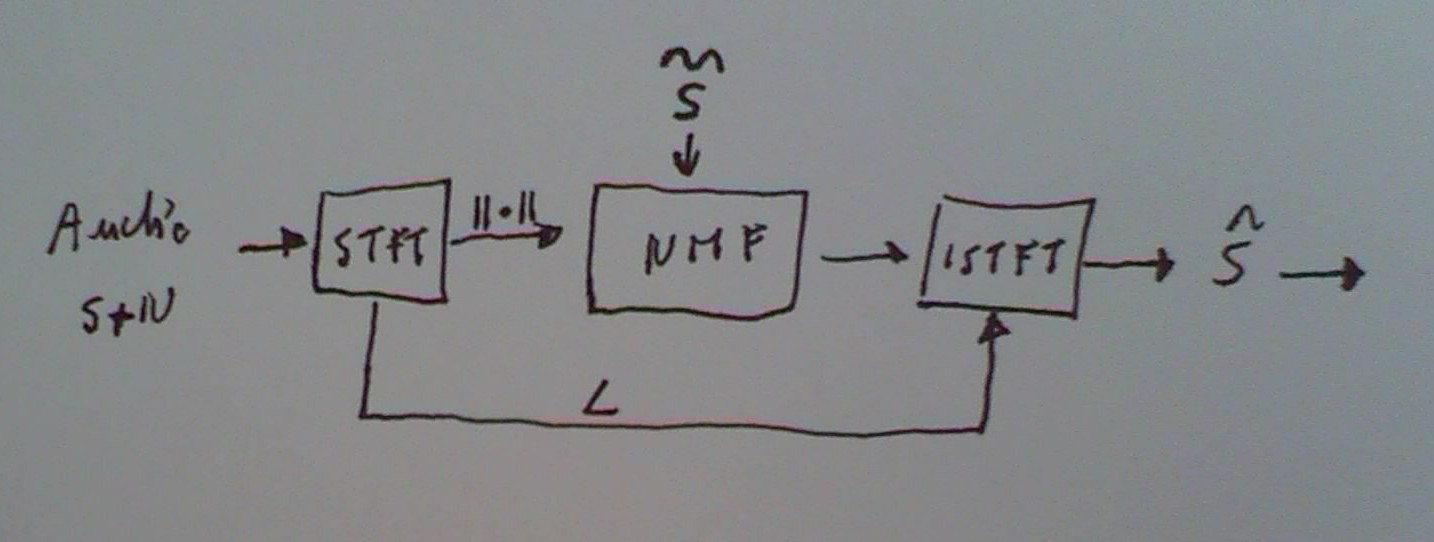
\includegraphics[width=.8\columnwidth]{figures/nmf}

NMF is an iterative scheme, do you set the number of iterations for balancing computational cost and performance ?
\end{center}
\end{block}
\end{frame}

\begin{frame}{Public horses for Source separation}
\begin{center}
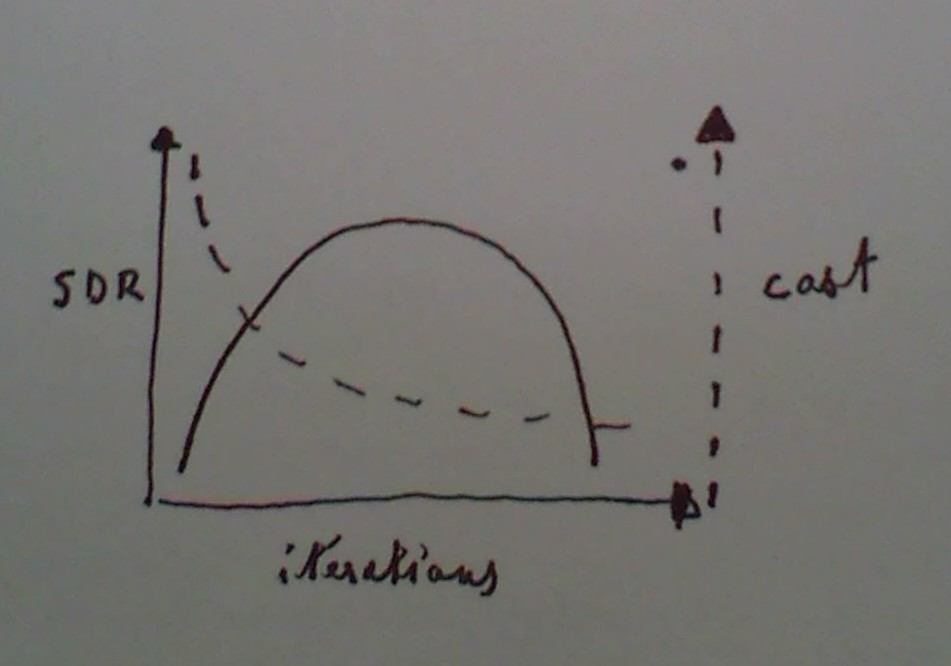
\includegraphics[width=.8\columnwidth]{figures/early}
\end{center}
\end{frame}


\begin{frame}{Public horses for Source separation}

\begin{block}{
the use of NMF is an example of a "public" horse}
\begin{itemize}
\item quality-of-fit optimized criterion
\item target criteria (SDR, SAR, SIR)
\item heavy use of "early stop" to ensure the non divergence of the target criteria
\end{itemize}
\end{block}
\end{frame}



\begin{frame}{Why hidden horses}

Digital data analysis is still in infancy (less than half a century), so uncontrolled behaviors are
\begin{itemize}
\item part of research
\item  and everyone is more or less happy with it
\end{itemize}
\end{frame}

\begin{frame}{Why hidden horses}

That said, spurious correlations are a well known matters in MANY, MANY, MANY research fields and the fact that the engineering community put so few effort on addressing those matters is childish. 

There are many ways our community is severely harming itself
\begin{itemize}
\item badly designed tasks
\item too small and biased datasets
\item unrealistic and non reproducible  results
\end{itemize}

\citenote{Warning Signs in Experimental Design and Interpretation}{http://norvig.com/experiment-design.html}{Peter Norvig:}{}
\end{frame}

\begin{frame}{An example}

\begin{block}{Acoustic Scene Similarity Retrieval (ASSR)}
\begin{center}
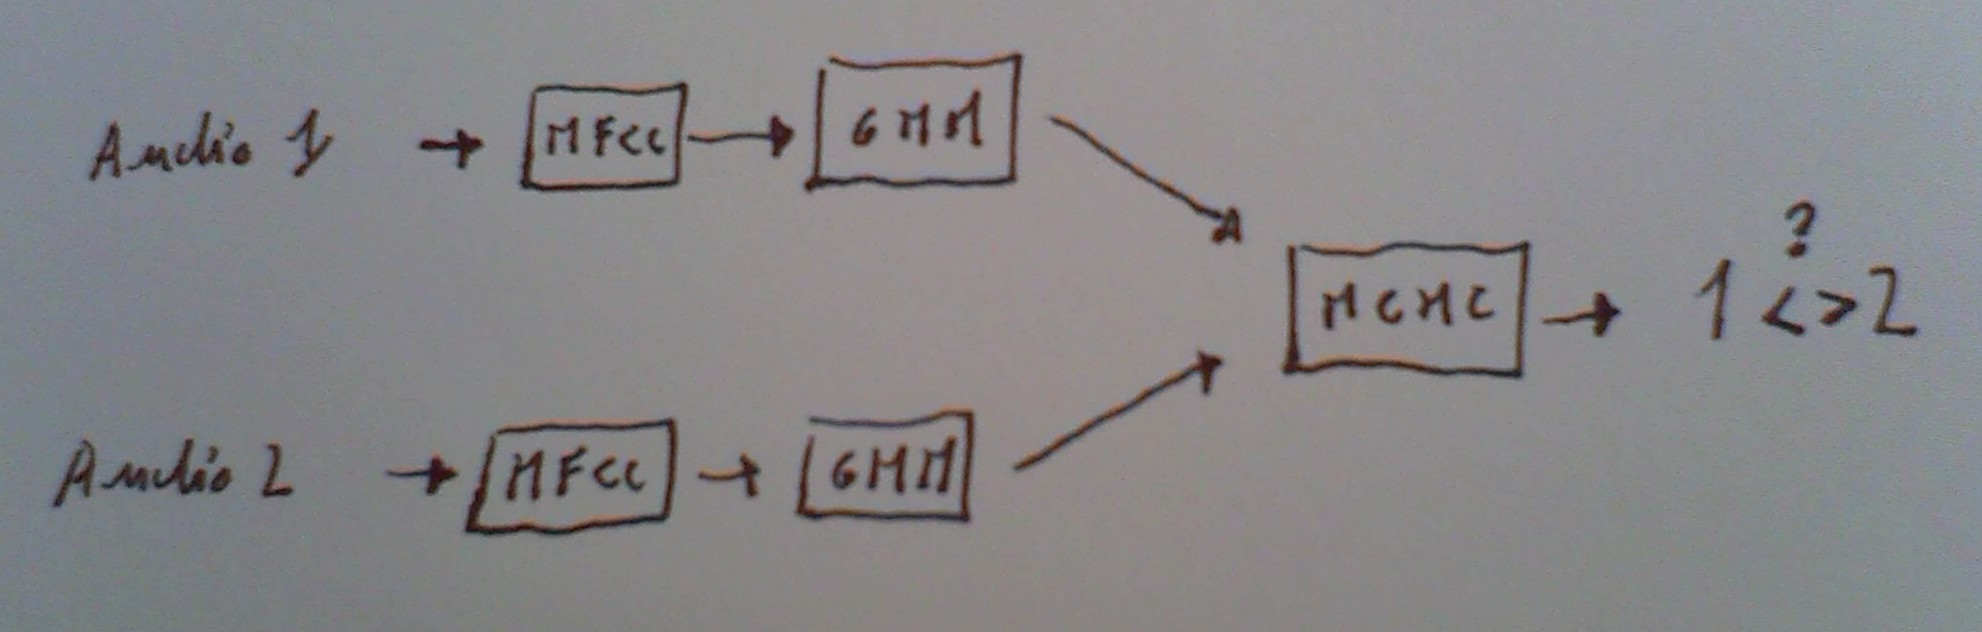
\includegraphics[width=\columnwidth]{figures/assr} \\
\end{center}
\end{block}

\end{frame}

\begin{frame}{An example}

\begin{block}{A Potemkin Village in ASSR}

\begin{itemize}
\item 2007: near perfect results, solved case
\item but strong issue in database design, similar to the album effect in artist / genre recognition
\item 2015: new figure, GMMs useless and performance only slightly over chance
\end{itemize}
\end{block}


\citenote{The bag-of-frames approach to audio pattern recognition: A sufficient model for urban soundscapes but not for polyphonic music}{https://scholar.google.fr/citations?view_op=view_citation&hl=fr&user=jnST06UAAAAJ&citation_for_view=jnST06UAAAAJ:UeHWp8X0CEIC}{J.J. Aucouturier \& al}{ The Journal of the Acoustical Society of America, 2007, vol. 122, no 2, p. 881-891}

\citenote{The bag-of-frames approach: a not so sufficient model for urban soundscapes}{http://scitation.aip.org/content/asa/journal/jasa/138/5/10.1121/1.4935350}{M. Lagrange \& al}{The Journal of the Acoustical Society of America, 2015, 138(5), EL487 - EL492}

\end{frame}

\section{SimScene}

\begin{frame}{One problem}
\begin{center}
\huge DATA
\end{center}
\end{frame}


\begin{frame}{Audio Scene Analysis}
\begin{center}
\begin{block}{We need}
\begin{itemize}
\item lots of data
\item well annotated data
\item public domain data
\item controllable complexity
\end{itemize}
\end{block}
\end{center}
\end{frame}

\begin{frame}{Data simulation}
\begin{center}
\begin{block}{IMHO}
\begin{itemize}
\item simulated data is ok, 
\item as long as the aim is to gain knowledge and not to go to production
\item simulation is not real data, but also not synthesized data
\item tricky part is to choose the right level of abstraction.
\end{itemize}
\end{block}
\end{center}
\end{frame}

\begin{frame}{SimScene}
\begin{center}

\includegraphics[width=.6\columnwidth]{figures/simscene} \\
\end{center}
\end{frame}


\begin{frame}{In a nutshell}
\begin{block}{SimScene is an acoustic scene simulator}
\begin{itemize}
\item built as a sequencer
\item with abstracted scheduling parameters
\item where events are defined as a set of recording samples
\item the outcome follows the "skeleton of events on a bed of texture paradigm" 
\end{itemize}
\end{block}

\citenote{An ear for statistics}{http://audition.ens.fr/adc/pdf/2013_NN_An_ear_for_statistics.pdf}{Nelken, I., \& de Cheveign\'e}{Nature neuroscience, 16(4), 381-382.}
\end{frame}


\begin{frame}{Use}
\begin{itemize}
\item Matlab
\item open source: \url{https://bitbucket.org/mlagrange/simscene}
\item used in DCASE 2013 and 2016 editions
\item produced datasets on archive
\end{itemize}
\citenote{An evaluation framework for event detection using a morphological model of acoustic scenes}{http://arxiv.org/abs/1502.00141}{Mathieu Lagrange, Gr\'egoire Lafay, Mathias Rossignol, Emmanouil Benetos, Axel Roebel}{IEEE TASLP v24-10, 1854-1864}
\end{frame}

\begin{frame}{Going deeper in performance analysis}
\begin{center}
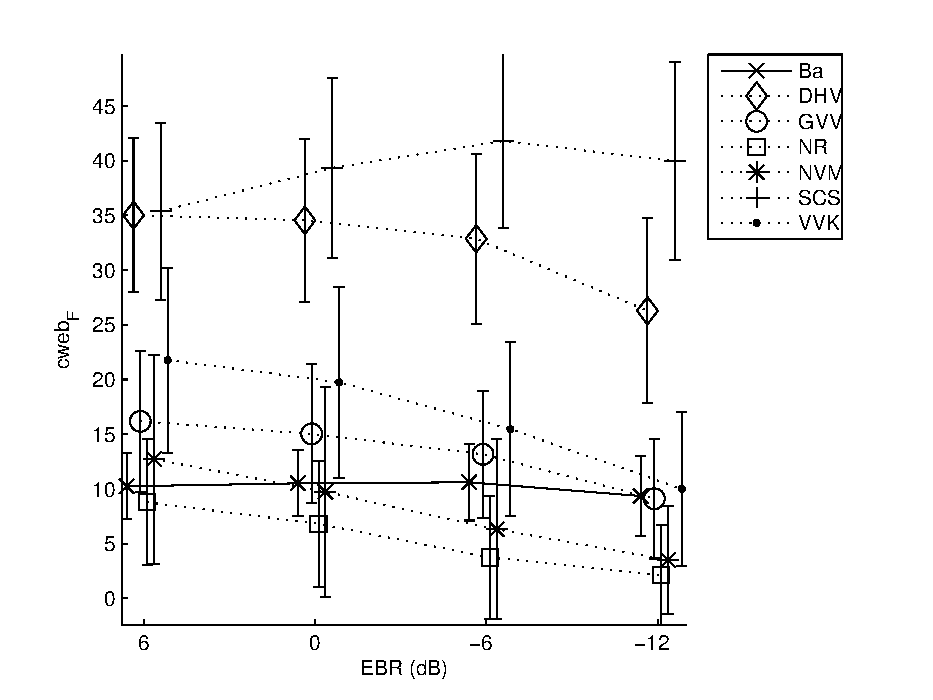
\includegraphics[width=.8\columnwidth]{../figures/ebr} \\
Varying Event to Background Ratio (EBR)
\end{center}
\end{frame}


\begin{frame}{Going deeper in performance analysis}
\begin{center}
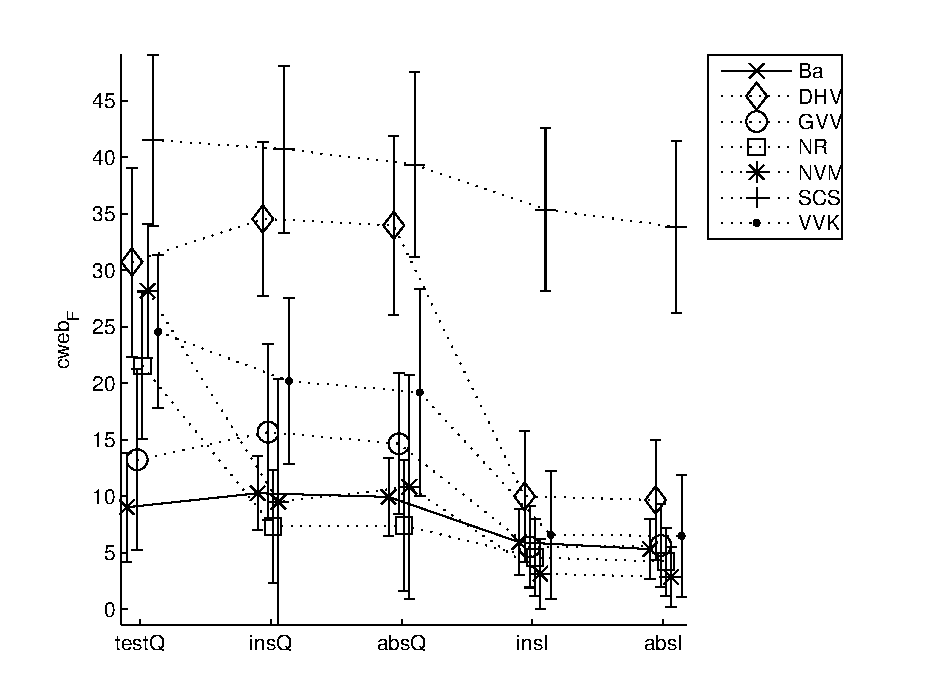
\includegraphics[width=.8\columnwidth]{../figures/irccyn} \\
Changing recording location for events and background
\end{center}
\end{frame}


\section{ExpLanes}

\begin{frame}{Another problem}
\begin{center}
\huge PROCESSING
\end{center}
\end{frame}

\begin{frame}{The scientific method}
\begin{itemize}
\item Analysis: Describe problem 
\item Hypothesis: Specify solution 
\item Synthesis: Implement solution 
\item Validation: Compute performance 
\end{itemize}
\end{frame}

\begin{frame}{Why using expLanes ?}
\begin{center}
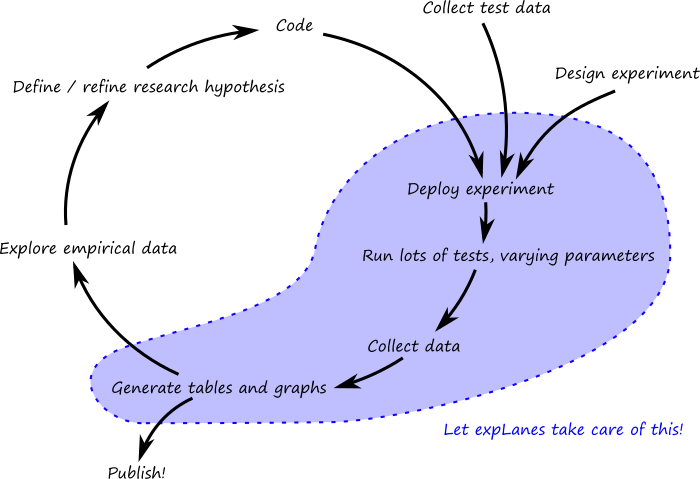
\includegraphics[width=.9\columnwidth]{figures/workflow} \\
\end{center}
\end{frame}

\begin{frame}{In a nutshell}
\begin{itemize}
\item Design: follow strictly the Design of Experiments paradigm (DoE)
\item Code: feed forward pipeline
\item Process: multi user, multi core, multi host
\item Reduce: fast and convenient thanks to factor masking
\item Visualize: Matlab, \LaTeX, html
\end{itemize}
\end{frame}

\begin{frame}{More}
\begin{itemize}
\item website : \url{http://mathieulagrange.github.io/expLanes}
\item demonstrations: clustering, source separation, ...
\item feedback welcome !
\end{itemize}
\end{frame}

\section{Reproducible Research}

\begin{frame}{Conclusions}
\begin{itemize}
\item The horse phenomenon is a reality
\item Potemkin villages are very common also in emerging fields
\item Scientists as individuals are smart humans
\item Yet, the social impact is very strong
\item As a community, the scientific method must be enforced
\item Strict reproducible research is the way to go
\item Need tools for that, not only languages
\end{itemize}
\end{frame}

\begin{frame}{Cathy O'Neil}
\begin{center}

\includegraphics[width=.4\columnwidth]{figures/maths}
\end{center}
\end{frame}

\begin{frame}{Lorena Barba}
\begin{center}

\includegraphics[width=.7\columnwidth]{figures/manifesto} \\
\url{https://figshare.com/articles/Reproducibility_PI_Manifesto/104539}
\end{center}
\end{frame}

\begin{frame}{Victoria Stodden}
\begin{center}
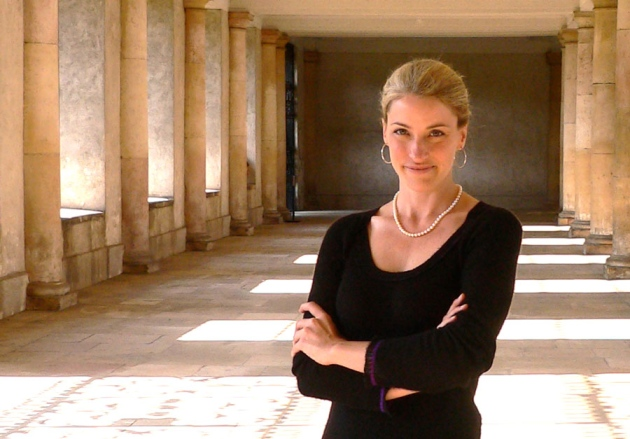
\includegraphics[width=.6\columnwidth]{figures/victoria}

one of three "reproducibility editors" appointed to look over code and data sets submitted by authors to the Journal of the American Statistical Association (JASA)
\end{center}

\end{frame}


\end{document}